\documentclass[12pt,a4paper]{article}
\usepackage[utf8]{inputenc}
\usepackage[T1]{fontenc}
\usepackage[polish]{babel}
\usepackage{amsmath}
\usepackage{graphicx}
\usepackage{hyperref}
\usepackage{geometry}
\usepackage{float}
\geometry{a4paper, margin=2.5cm}

\title{Sprawozdanie: Klasyczny Algorytm Genetyczny}
\author{Jakub Balicki}
\date{\today}

\begin{document}

\maketitle

\section*{Link do repozytorium}
\url{https://github.com/balicz3k/GeneticAlgorithm}

\section{Technologie użyte w projekcie}
Projekt został zrealizowany w języku \textbf{Python}. Do stworzenia autorskiego i nowoczesnego interfejsu graficznego (GUI) wykorzystano bibliotekę \textbf{CustomTkinter}. Złożone operacje matematyczne oparto na bibliotekach \textbf{NumPy} oraz \textbf{SciPy}. Wyniki działania algorytmu zostały zwizualizowane za pomocą biblioteki \textbf{Matplotlib}, a agregacja i modyfikacja danych przeprowadzona z użyciem \textbf{Pandas}.

\section{Wygląd aplikacji}
\begin{figure}[H]
    \centering
    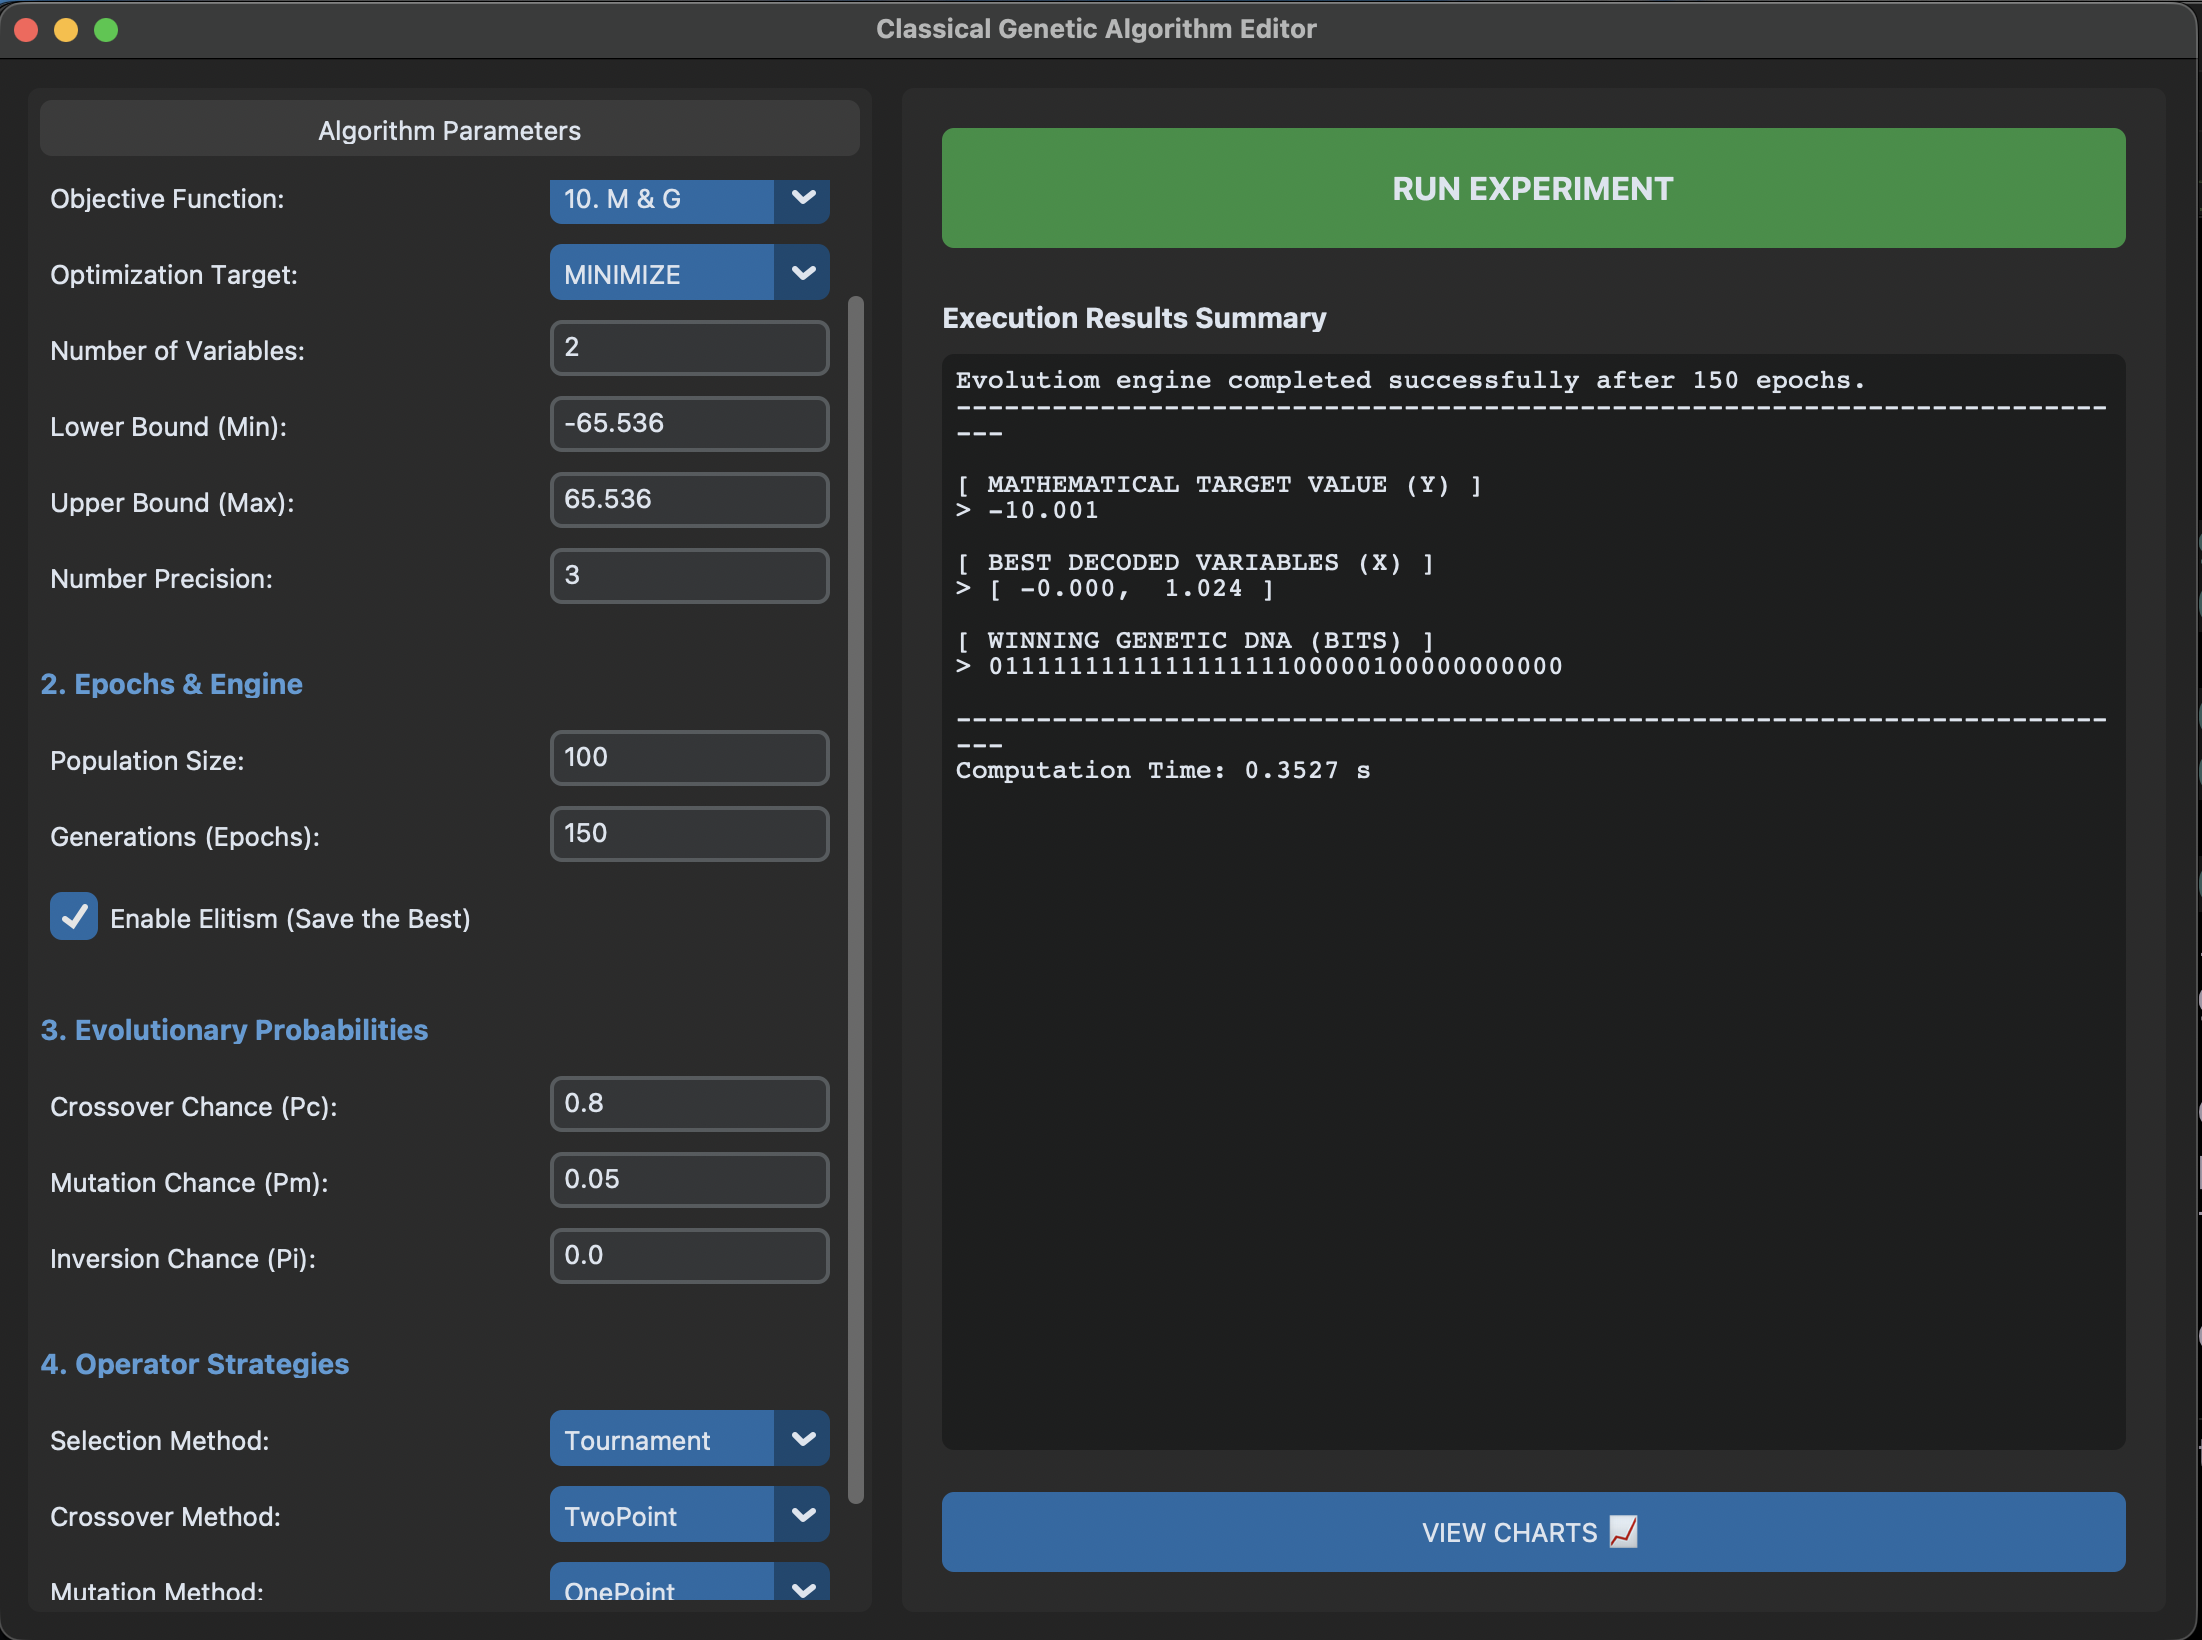
\includegraphics[width=0.85\textwidth]{img/basic_view.png}
    \caption{Interfejs główny aplikacji – panel kontrolny.}
    \label{fig:basic}
\end{figure}

\begin{figure}[H]
    \centering
    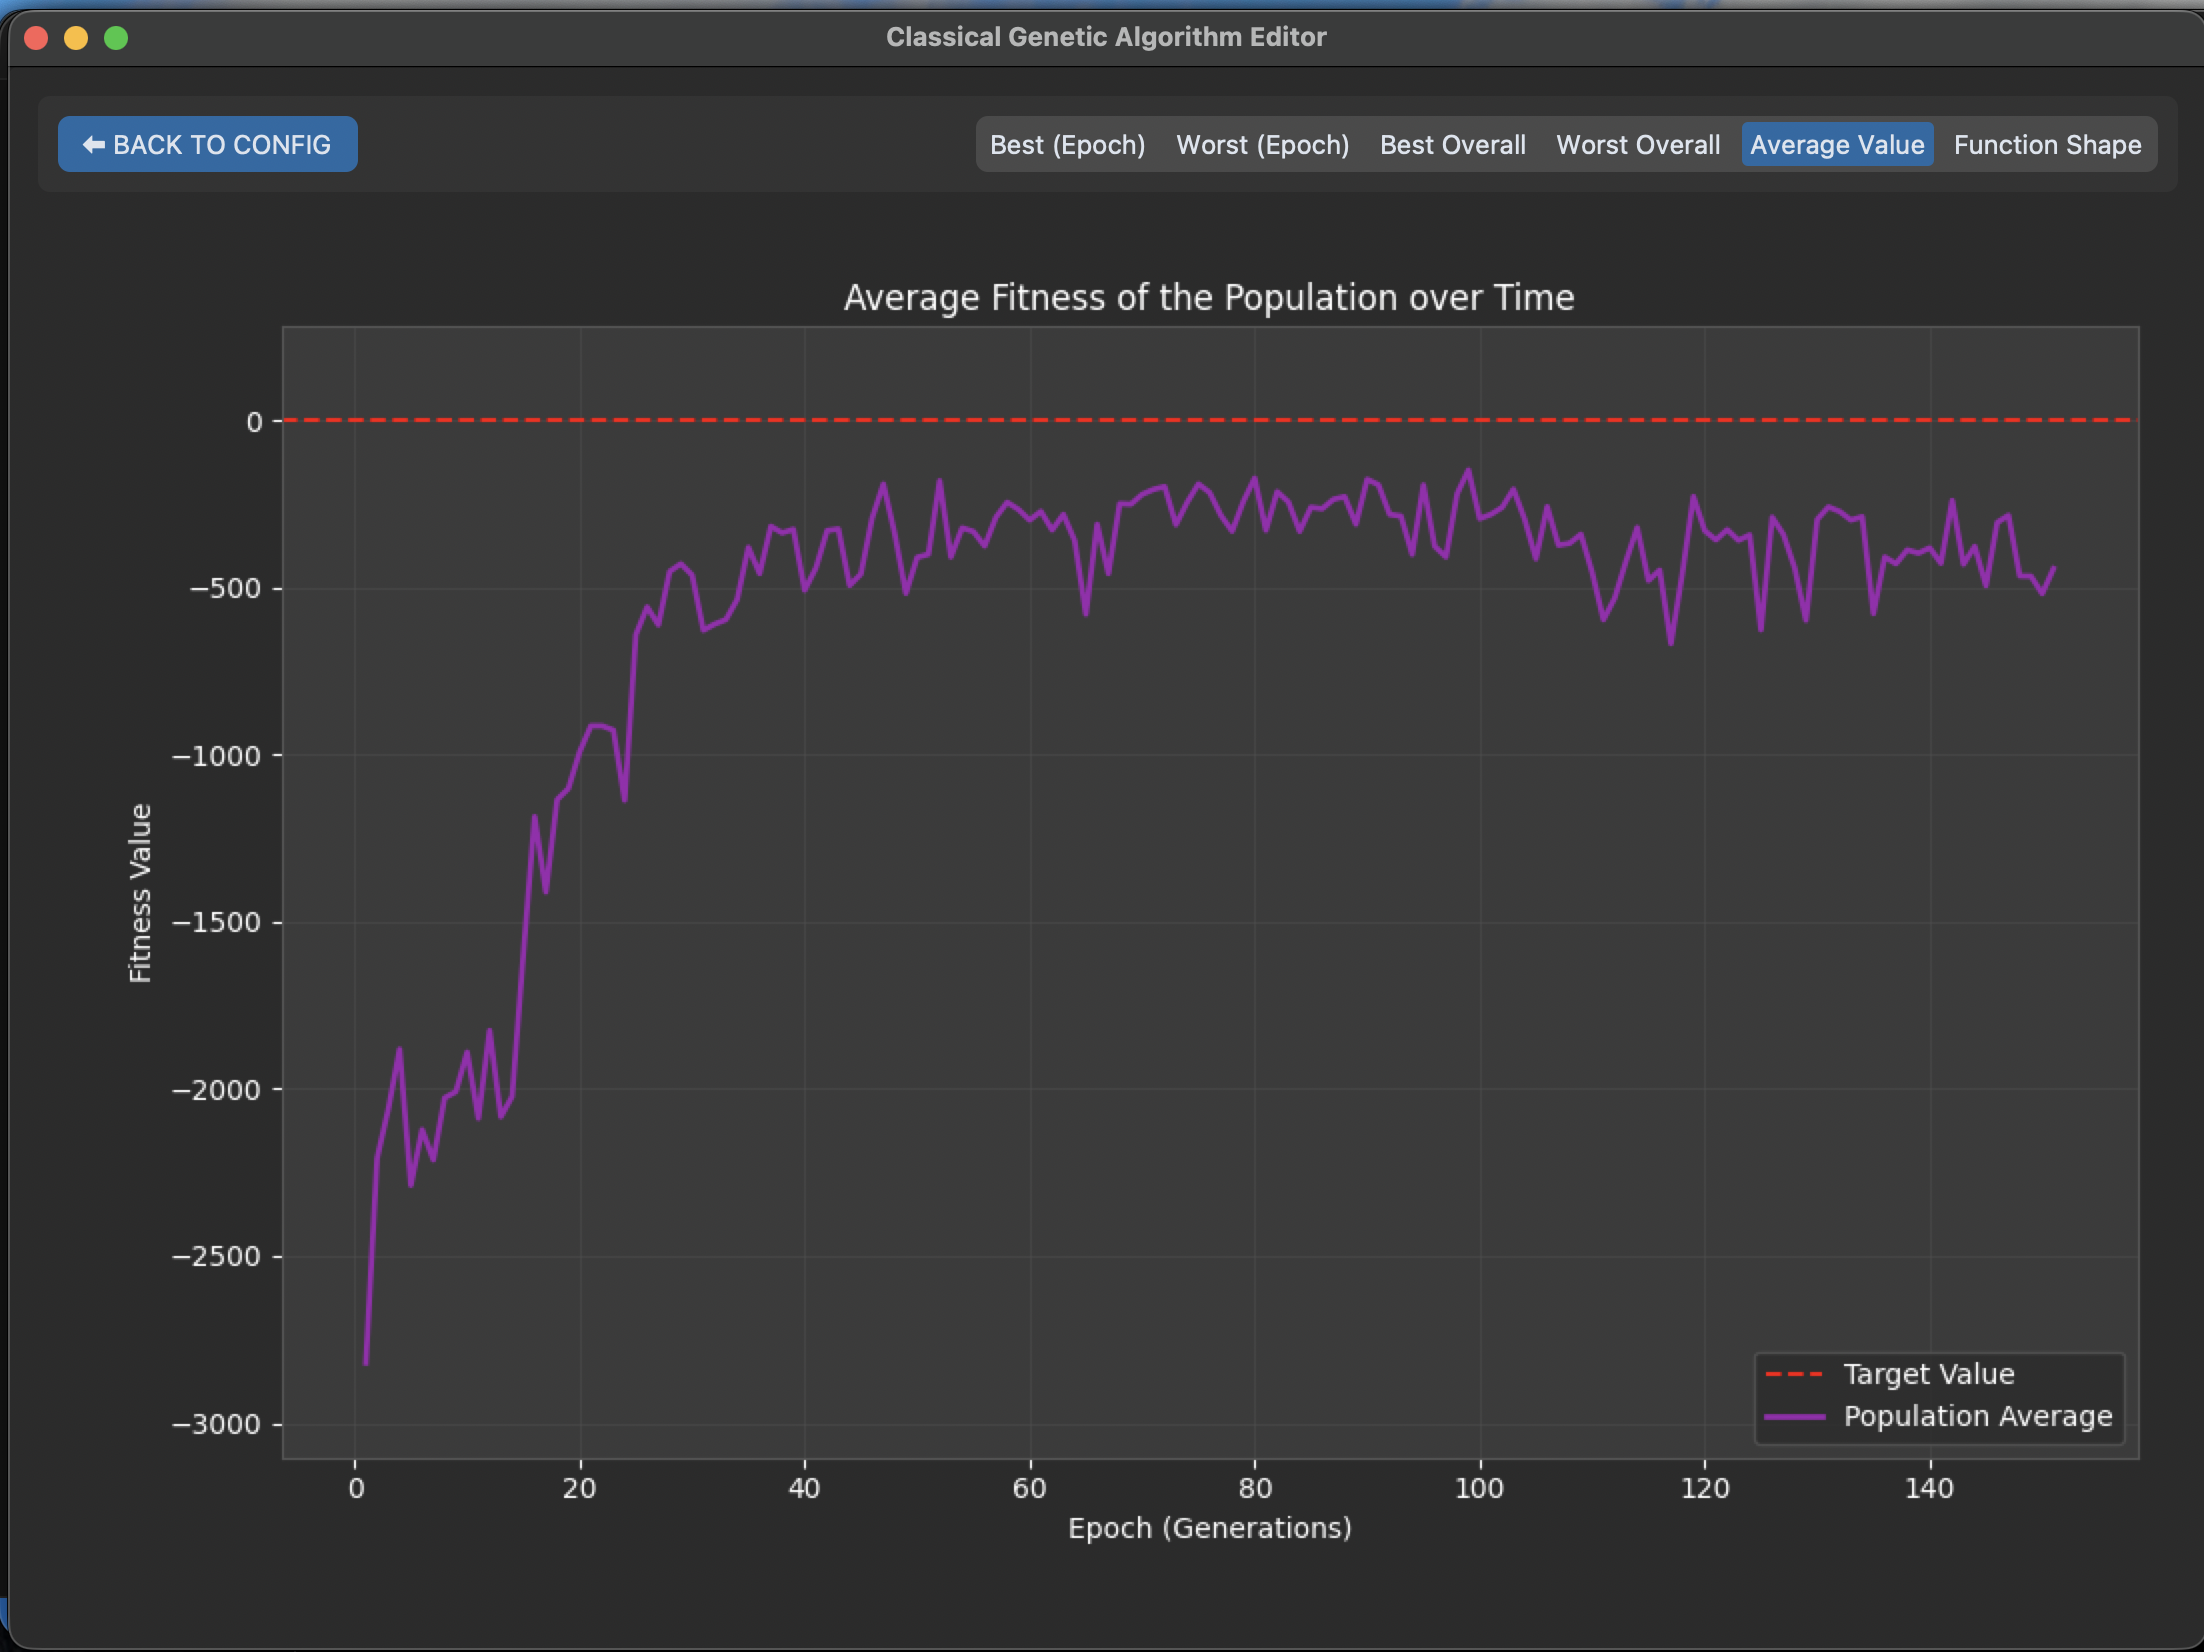
\includegraphics[width=0.85\textwidth]{img/chart_view.png}
    \caption{Podgląd dynamicznego wykresu w oparciu o zebrane pomiary procesu ewolucyjnego programu.}
    \label{fig:chart}
\end{figure}

\section{Porównanie wyników dla różnych konfiguracji algorytmu}
Badane wyniki wskazują jednoznacznie zachowanie algorytmu w odniesieniu do prawdopodobieństwa i rozmiarów mutacji, a także inwersji oraz siły z jaką krzyżowane są osobniki. 
\begin{itemize}
    \item \textbf{Częstotliwość krzyżowania:} Wyższe prawdobodobieństwo (rzędu $0.7 - 0.9$) znacznie podnosi tempo dążenia do minimum, jednak w wypadku funkcji mocno wielomodalnych szybko zawęża pulę genów do jednego, przedwczesnego lokalnego minimum.
    \item \textbf{Współczynnik mutacji:} Małe, rzadkie mutacje (np $p=0.01$) dobrze stabilizują zbieganie po znalezieniu rejonów docelowych. Zbyt silna mutacja ($p>0.2$) przerodziła poszukiwania w metodę czysto losową.
    \item \textbf{Elita:} Pozostawienie najlepszych wektorów między populacjami ma kluczowe znaczenie przy zachowaniu postępu, unikając spadku efektywności wywoływanego silnymi operacjami.
\end{itemize}
\end{document}
